% Editable native annotations around unchanged verified IDE photographs.
\par
\begin{figure}[htbp]
\centering
\sbox0{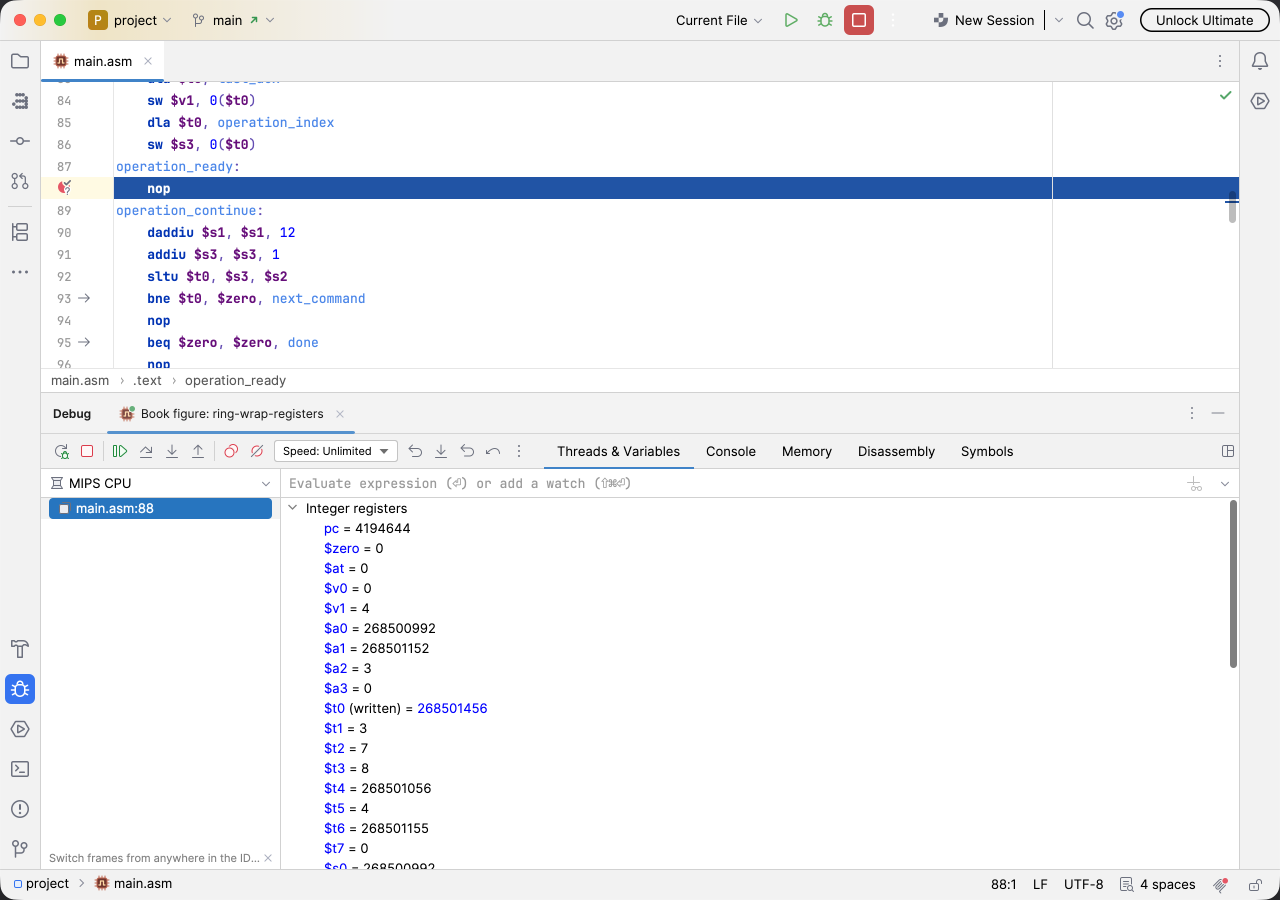
\includegraphics[artifact]{packages/014-ring-buffer-logger/captures/f01-wrap/registers.png}}
\sbox2{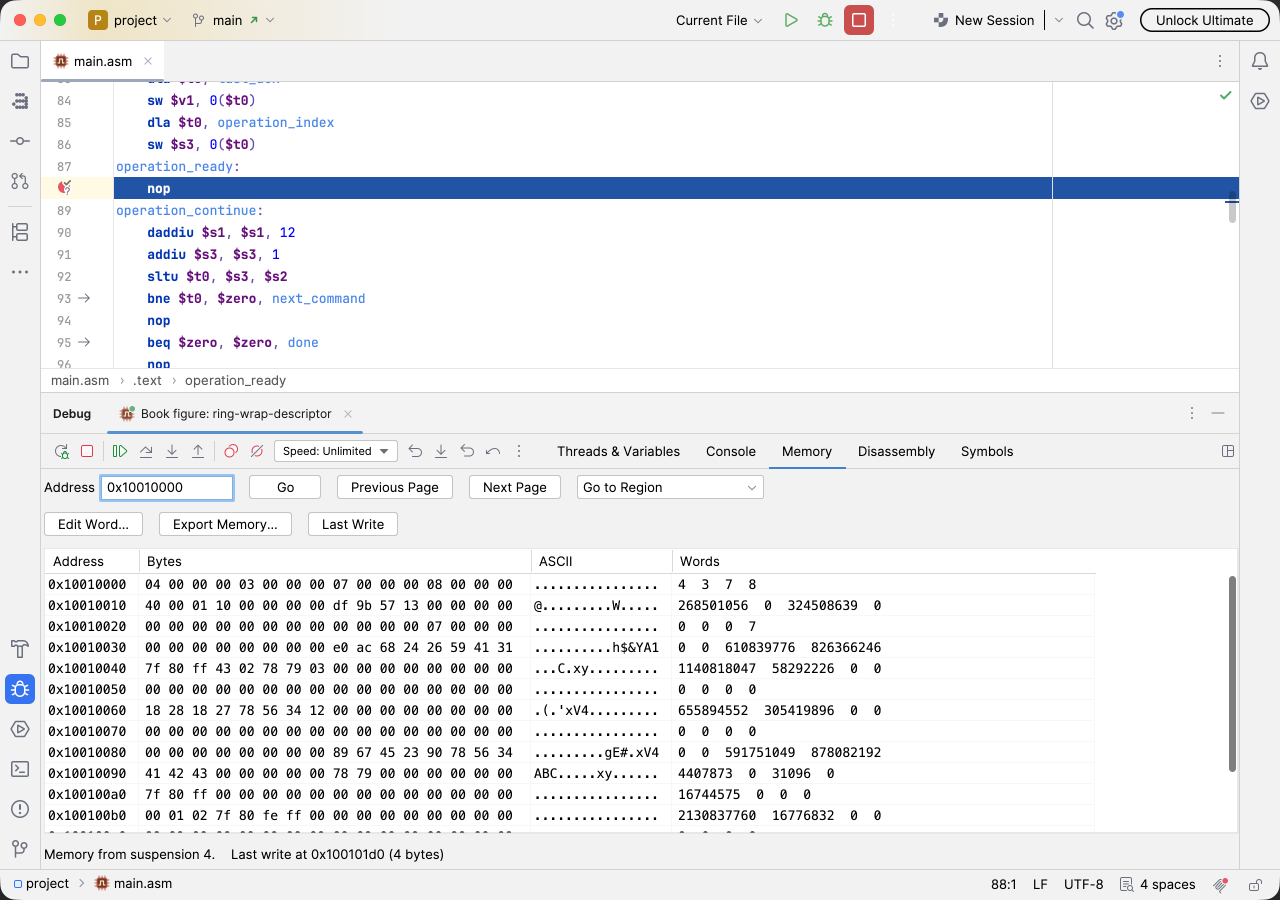
\includegraphics[artifact]{packages/014-ring-buffer-logger/captures/f01-wrap/descriptor.png}}
\sbox4{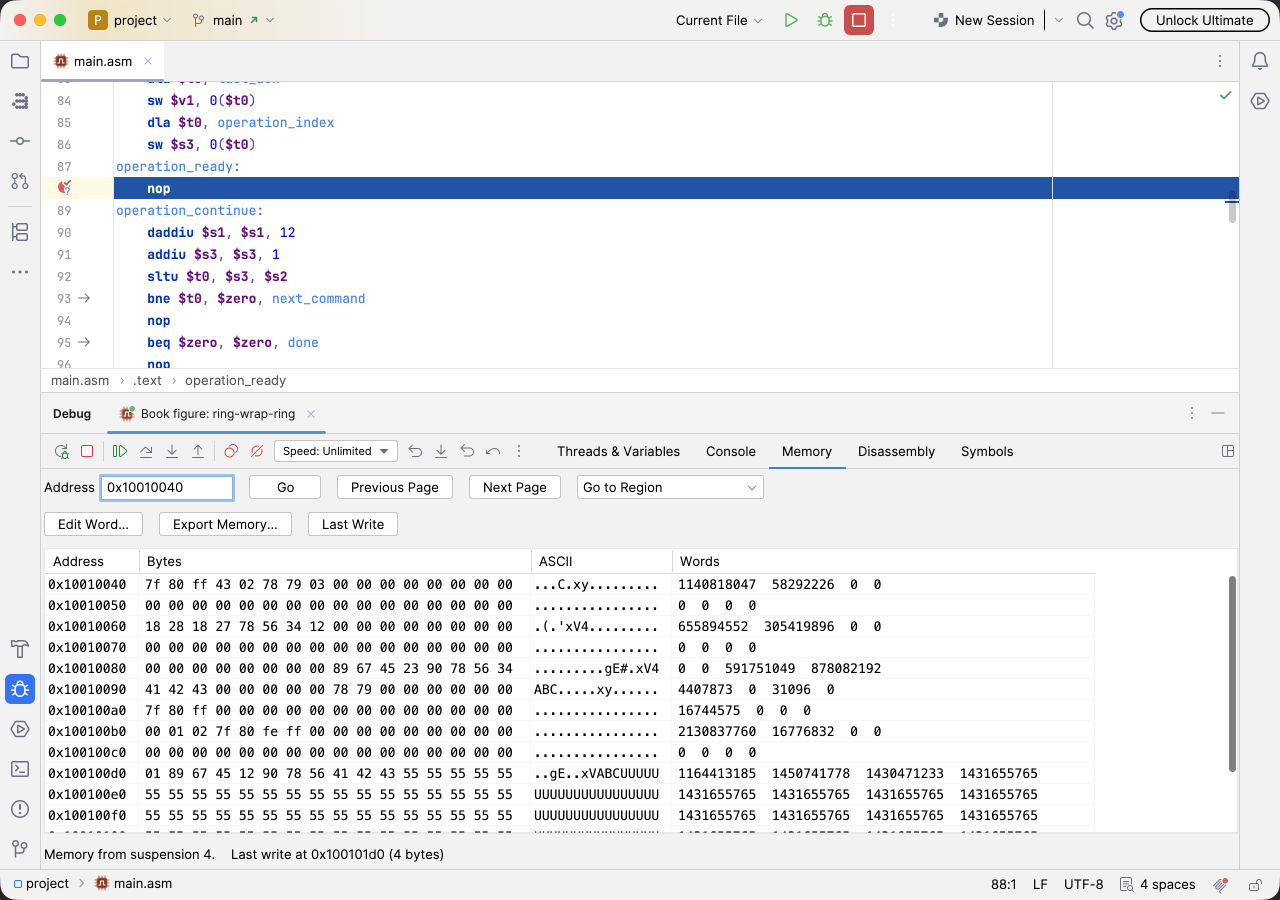
\includegraphics[artifact]{packages/014-ring-buffer-logger/captures/f01-wrap/ring.png}}
\sbox6{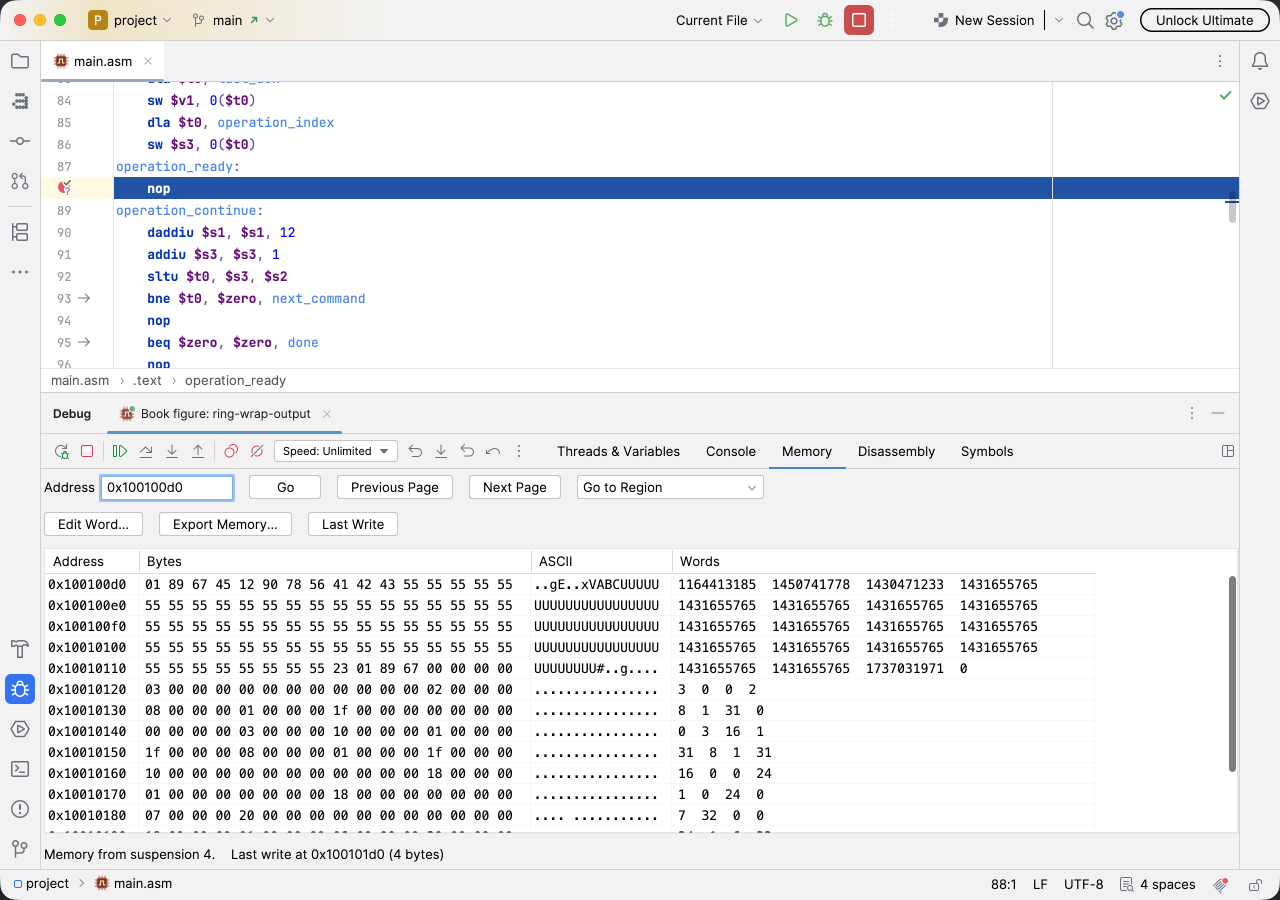
\includegraphics[artifact]{packages/014-ring-buffer-logger/captures/f01-wrap/output.png}}
\edef\MARSringwrapsourceLeft{\the\dimexpr0.036718750\wd0\relax}
\edef\MARSringwrapsourceBottom{\the\dimexpr0.774444444\ht0\relax}
\edef\MARSringwrapsourceRight{\the\dimexpr0.713281250\wd0\relax}
\edef\MARSringwrapsourceTop{\the\dimexpr0.147777778\ht0\relax}
\edef\MARSringwrapregistersLeft{\the\dimexpr0.246093750\wd0\relax}
\edef\MARSringwrapregistersBottom{\the\dimexpr0.312222222\ht0\relax}
\edef\MARSringwrapregistersRight{\the\dimexpr0.553906250\wd0\relax}
\edef\MARSringwrapregistersTop{\the\dimexpr0.640000000\ht0\relax}
\edef\MARSringwrapdescriptorLeft{\the\dimexpr0.034375000\wd2\relax}
\edef\MARSringwrapdescriptorBottom{\the\dimexpr0.311111111\ht2\relax}
\edef\MARSringwrapdescriptorRight{\the\dimexpr0.584375000\wd2\relax}
\edef\MARSringwrapdescriptorTop{\the\dimexpr0.608888889\ht2\relax}
\edef\MARSringwrapringLeft{\the\dimexpr0.034375000\wd4\relax}
\edef\MARSringwrapringBottom{\the\dimexpr0.334444444\ht4\relax}
\edef\MARSringwrapringRight{\the\dimexpr0.584375000\wd4\relax}
\edef\MARSringwrapringTop{\the\dimexpr0.608888889\ht4\relax}
\edef\MARSringwrapoutputLeft{\the\dimexpr0.034375000\wd6\relax}
\edef\MARSringwrapoutputBottom{\the\dimexpr0.311111111\ht6\relax}
\edef\MARSringwrapoutputRight{\the\dimexpr0.584375000\wd6\relax}
\edef\MARSringwrapoutputTop{\the\dimexpr0.608888889\ht6\relax}
\begin{tikzpicture}[alt={Five annotated details after command index three. The next instruction is operation ready. Return status is zero and encoded size is four. Descriptor head four, tail three, used seven and capacity eight accompany the full ring pointer. At physical indices four through seven and zero through two, records contain x y and hexadecimal 7f 80 ff. Old byte 43 at index three is unoccupied. Output contains the earlier popped A B C.}]
\node[anchor=north west,inner sep=0,font=\small\bfseries] (source-title) at (6mm,0) {Next instruction after publication};
\node[anchor=north west,inner sep=0] (source) at ([yshift=-1mm]source-title.south west) {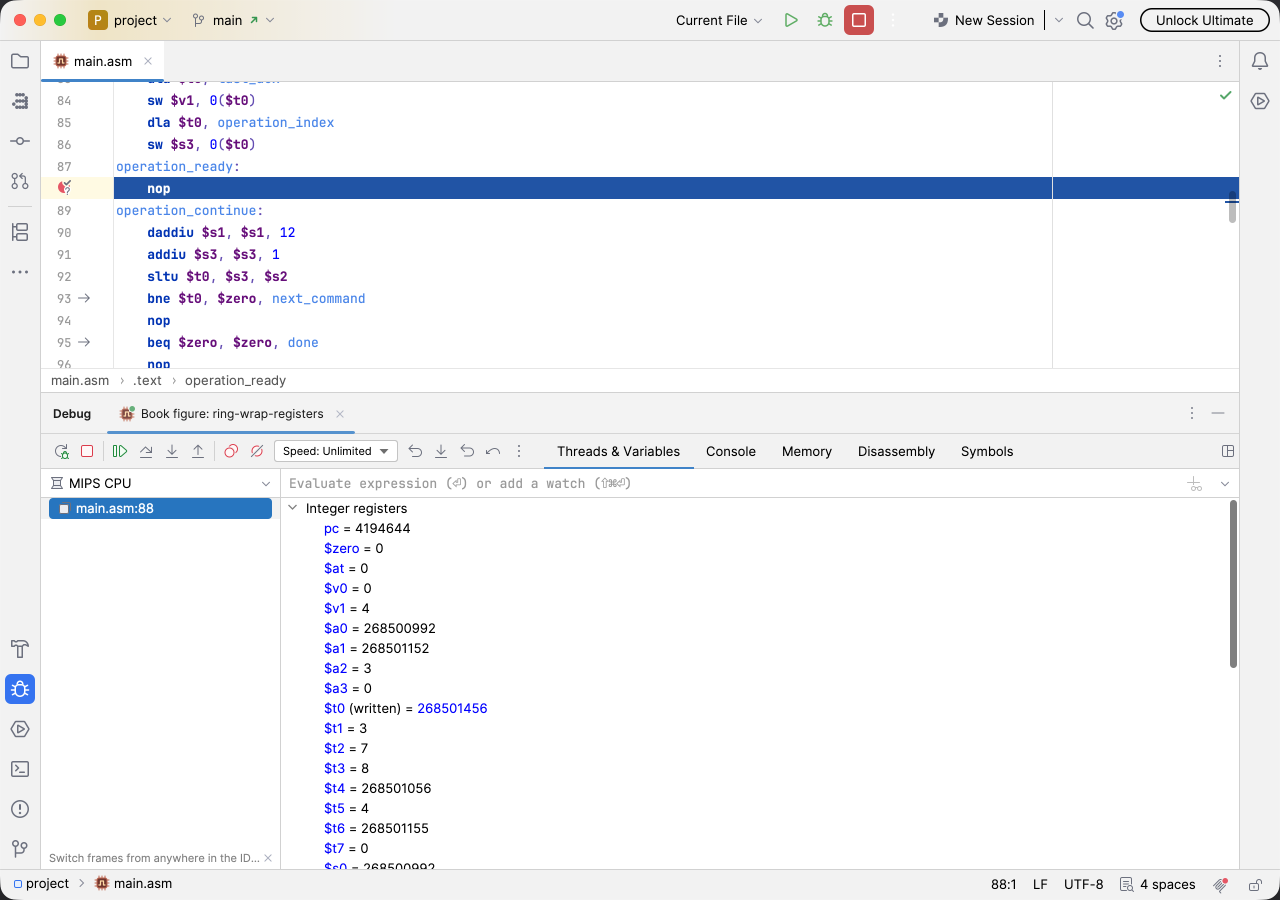
\includegraphics[width=0.54\linewidth,artifact,trim={\MARSringwrapsourceLeft{} \MARSringwrapsourceBottom{} \MARSringwrapsourceRight{} \MARSringwrapsourceTop{}},clip]{packages/014-ring-buffer-logger/captures/f01-wrap/registers.png}};
\begin{scope}[shift={(source.south west)},x={($(source.south east)-(source.south west)$)},y={($(source.north west)-(source.south west)$)}]
\draw[black,line width=0.7pt] (0.215625000,0.057142857) rectangle (0.384375000,0.371428571);
\node[draw=black,fill=white,circle,inner sep=1.5pt,font=\footnotesize] at ($(0.215625000,0.371428571)+(-3mm,0)$) {1};
\end{scope}
\node[anchor=north west,inner sep=0,font=\small\bfseries] (registers-title) at (0.58\linewidth,0 |- source-title.north) {Signed return values};
\node[anchor=north west,inner sep=0] (registers) at ([yshift=-1mm]registers-title.south west) {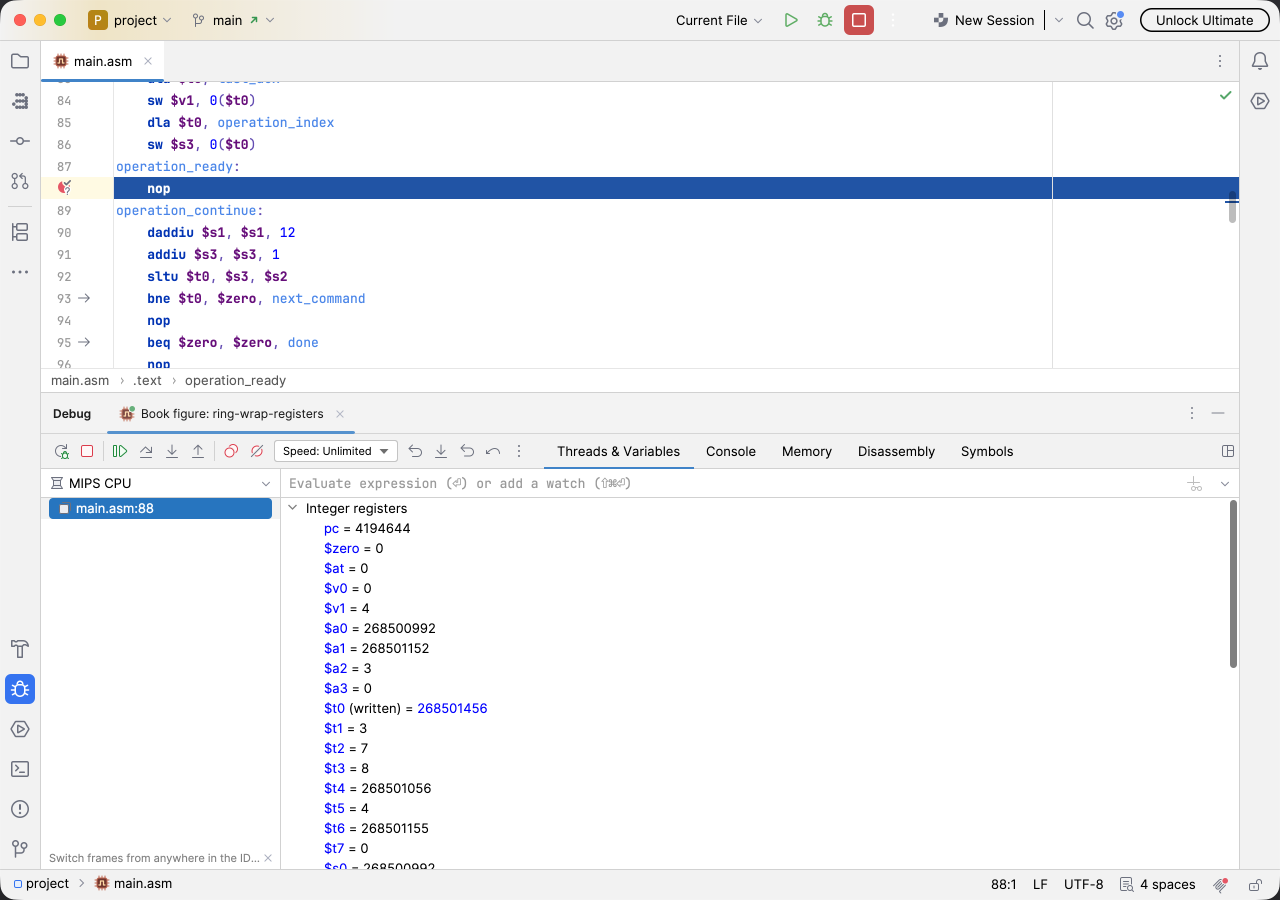
\includegraphics[width=0.42\linewidth,artifact,trim={\MARSringwrapregistersLeft{} \MARSringwrapregistersBottom{} \MARSringwrapregistersRight{} \MARSringwrapregistersTop{}},clip]{packages/014-ring-buffer-logger/captures/f01-wrap/registers.png}};
\begin{scope}[shift={(registers.south west)},x={($(registers.south east)-(registers.south west)$)},y={($(registers.north west)-(registers.south west)$)}]
\draw[black,line width=0.7pt] (0.023437500,0.023255814) rectangle (0.226562500,0.953488372);
\node[draw=black,fill=white,circle,inner sep=1.5pt,font=\footnotesize] at ($(0.023437500,0.953488372)+(-3mm,0)$) {2};
\end{scope}
\node[anchor=north west,inner sep=0,font=\small\bfseries] (descriptor-title) at ([yshift=-3mm]source.south west) {Descriptor words and full buffer pointer};
\node[anchor=north west,inner sep=0] (descriptor) at ([yshift=-1mm]descriptor-title.south west) {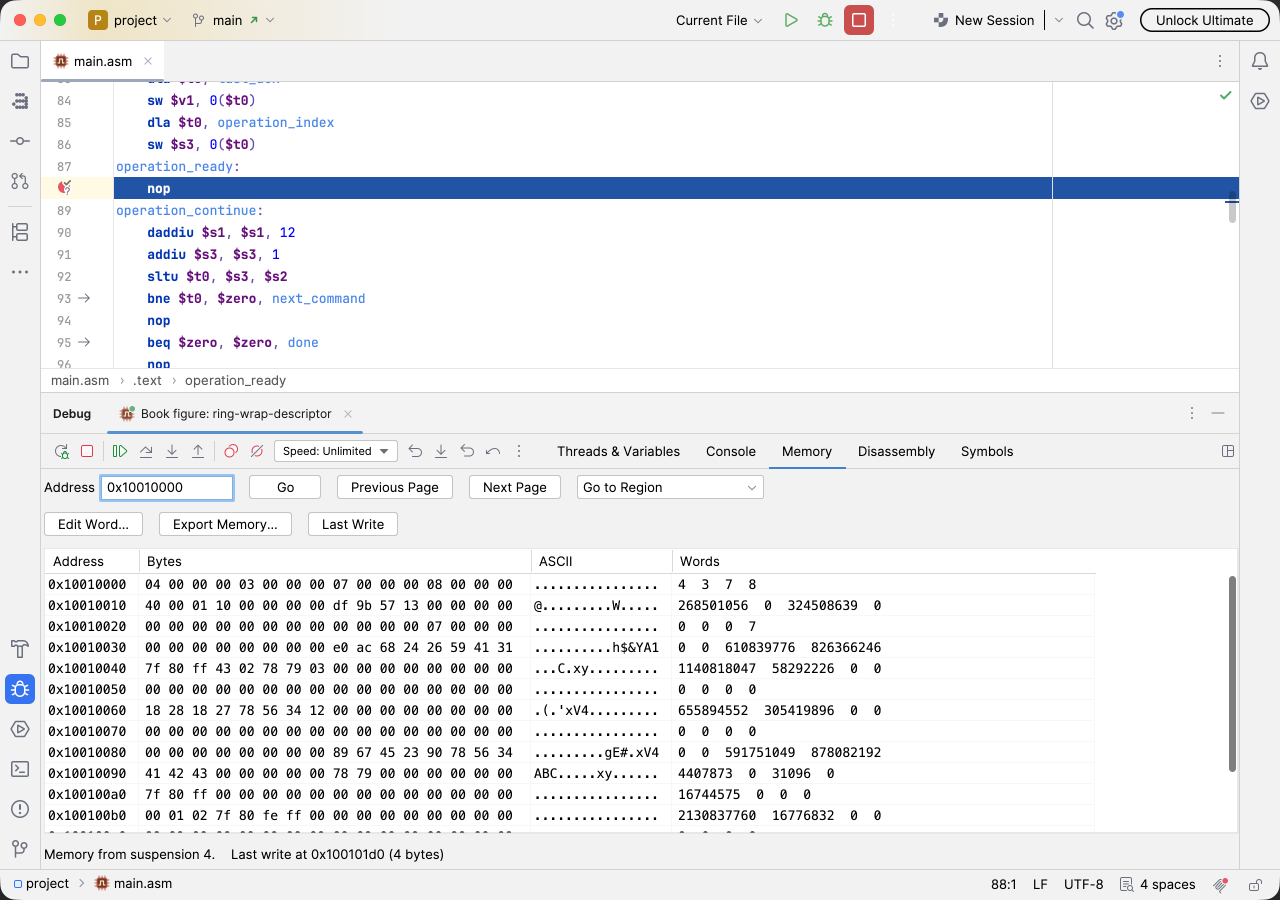
\includegraphics[width=0.84\linewidth,artifact,trim={\MARSringwrapdescriptorLeft{} \MARSringwrapdescriptorBottom{} \MARSringwrapdescriptorRight{} \MARSringwrapdescriptorTop{}},clip]{packages/014-ring-buffer-logger/captures/f01-wrap/descriptor.png}};
\begin{scope}[shift={(descriptor.south west)},x={($(descriptor.south east)-(descriptor.south west)$)},y={($(descriptor.north west)-(descriptor.south west)$)}]
\draw[black,line width=0.7pt] (0.194672131,0.055555556) rectangle (0.997950820,0.638888889);
\node[draw=black,fill=white,circle,inner sep=1.5pt,font=\footnotesize] at ($(0,0.638888889)+(-3mm,0)$) {3};
\end{scope}
\node[anchor=north west,inner sep=0,font=\small\bfseries] (ring-title) at ([yshift=-3mm]descriptor.south west) {Physical ring bytes, including mapped padding};
\node[anchor=north west,inner sep=0] (ring) at ([yshift=-1mm]ring-title.south west) {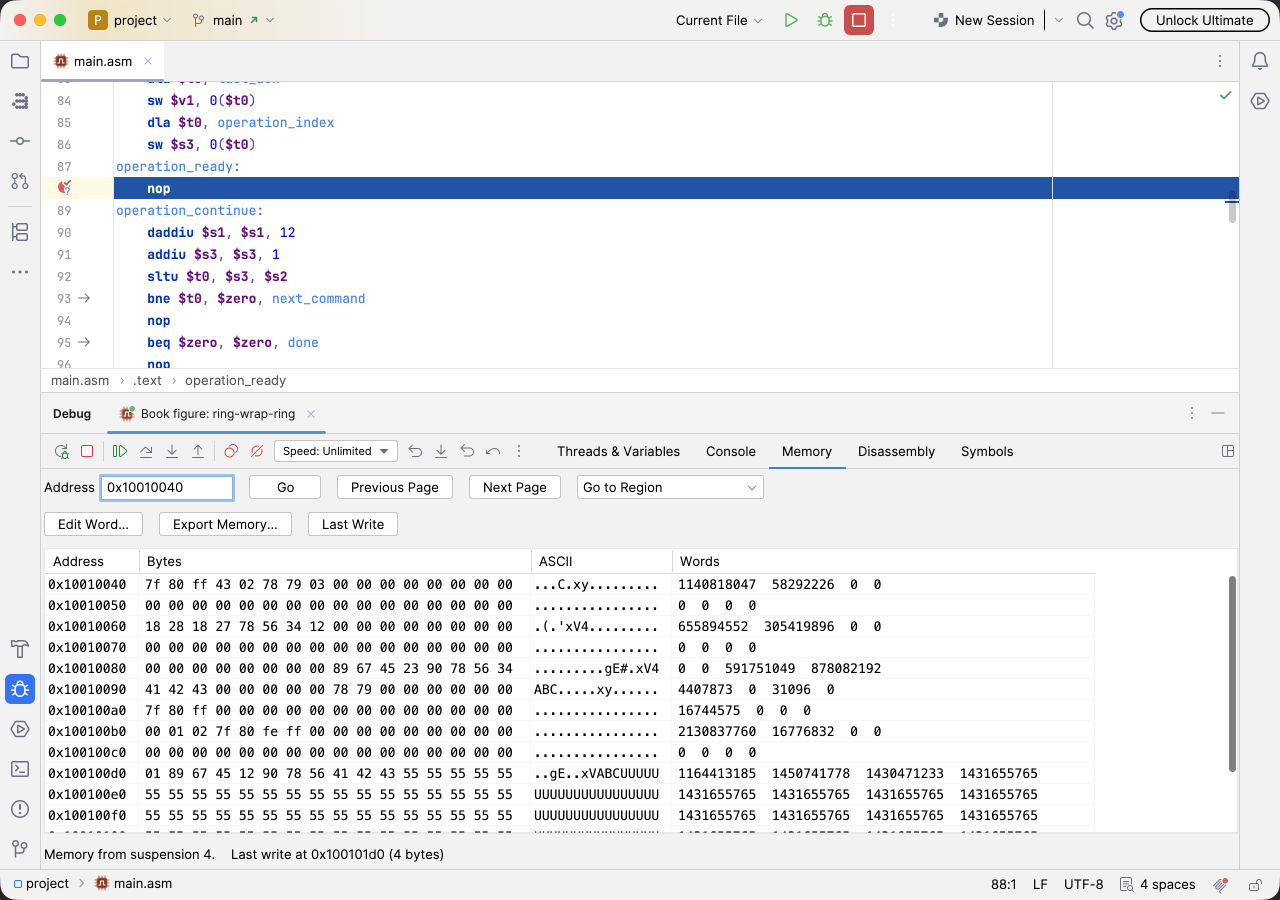
\includegraphics[width=0.84\linewidth,artifact,trim={\MARSringwrapringLeft{} \MARSringwrapringBottom{} \MARSringwrapringRight{} \MARSringwrapringTop{}},clip]{packages/014-ring-buffer-logger/captures/f01-wrap/ring.png}};
\begin{scope}[shift={(ring.south west)},x={($(ring.south east)-(ring.south west)$)},y={($(ring.north west)-(ring.south west)$)}]
\draw[black,line width=0.7pt] (0.194672131,0.078431373) rectangle (0.997950820,0.490196078);
\node[draw=black,fill=white,circle,inner sep=1.5pt,font=\footnotesize] at ($(0,0.490196078)+(-3mm,0)$) {4};
\end{scope}
\node[anchor=north west,inner sep=0,font=\small\bfseries] (output-title) at ([yshift=-3mm]ring.south west) {Output bytes and neighboring objects};
\node[anchor=north west,inner sep=0] (output) at ([yshift=-1mm]output-title.south west) {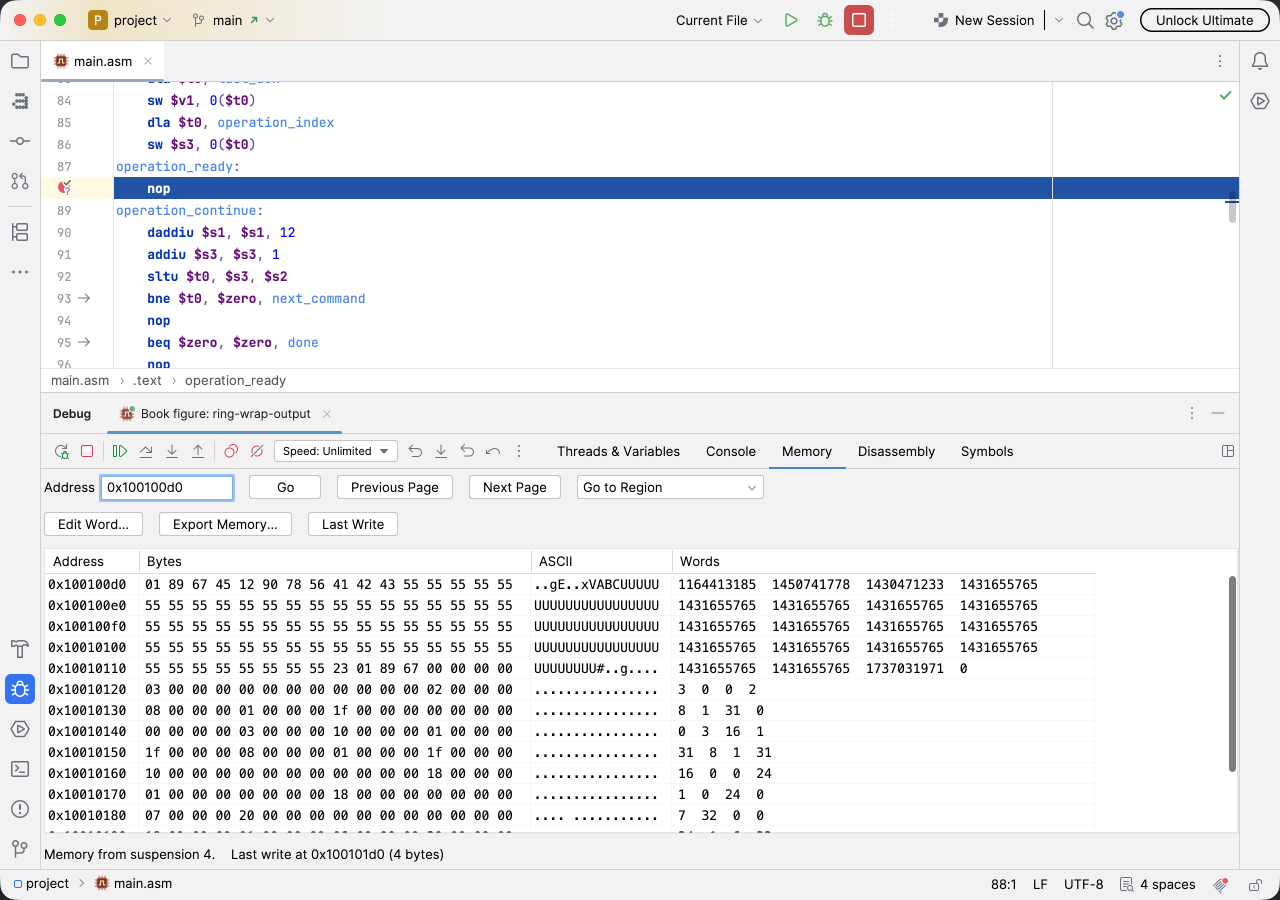
\includegraphics[width=0.84\linewidth,artifact,trim={\MARSringwrapoutputLeft{} \MARSringwrapoutputBottom{} \MARSringwrapoutputRight{} \MARSringwrapoutputTop{}},clip]{packages/014-ring-buffer-logger/captures/f01-wrap/output.png}};
\begin{scope}[shift={(output.south west)},x={($(output.south east)-(output.south west)$)},y={($(output.north west)-(output.south west)$)}]
\draw[black,line width=0.7pt] (0.194672131,0.055555556) rectangle (0.997950820,0.638888889);
\node[draw=black,fill=white,circle,inner sep=1.5pt,font=\footnotesize] at ($(0,0.638888889)+(-3mm,0)$) {5};
\end{scope}
\end{tikzpicture}
\par\smallskip
\begin{minipage}{\linewidth}
\small
\begin{enumerate}
\setlength{\itemsep}{2pt}
\setlength{\parsep}{0pt}
\item The blue \texttt{nop} at \texttt{operation\_ready} is next after command index 3, the fourth command. The call has returned and the caller has published its results. Each panel replays this same unchanged program to the conditional breakpoint \texttt{\$s3 == 3}.
\item The native signed-decimal registers show \texttt{\$v0 = 0}: push succeeded. \texttt{\$v1 = 4} counts the one-byte length prefix and three-byte payload inserted by this call. The return values describe this operation, while the descriptor counts everything still queued.
\item The first line contains four little-endian words: head 4, tail 3, used 7 and capacity 8. The next line starts with eight pointer bytes \texttt{40 00 01 10 00 00 00 00}, or \texttt{0x10010040}. The following guard and alignment padding are outside the descriptor. Seven occupied bytes leave one free byte.
\item Only the first eight bytes of the ring row belong to this capacity-eight queue. Start at head index 4: \texttt{02 78 79} encodes the two-byte record \texttt{xy}. Its successor begins at index 7: prefix \texttt{03} is followed by \texttt{7f 80 ff} at indices 0, 1 and 2. Tail index 3 names the next free slot; its stale \texttt{43} byte is not queued data.
\item The output allocation begins at \texttt{0x100100d8}, eight bytes into the first displayed row. Bytes \texttt{41 42 43} are \texttt{ABC}, removed by the preceding pop. The next push does not change them. The leading eight displayed bytes are guards; subsequent \texttt{55} bytes are untouched output. Removing a record did not erase its former ring bytes.
\end{enumerate}
\end{minipage}
\caption{Two queued records span the physical end of the eight-byte ring.}
\label{capture:014-ring-buffer-logger-f01-wrap}
\label{ring-f01-wrap}
\end{figure}
\par
